\documentclass[12pt,a4paper]{article}

% ─── Page Layout ───────────────────────────────────────────────────────────────
\usepackage[a4paper, margin=0.8in, headheight=14pt]{geometry}

% ─── Fonts (XeLaTeX) ───────────────────────────────────────────────────────────
\usepackage{fontspec}
\usepackage{unicode-math}
\setmainfont{TeX Gyre Pagella}
\setmonofont[Scale=0.88]{TeX Gyre Cursor}
\setmathfont{Latin Modern Math}

% ─── Packages ──────────────────────────────────────────────────────────────────
\usepackage{xcolor}
\usepackage{colortbl}
\usepackage{titlesec}
\usepackage{enumitem}
\usepackage{tabularx}
\usepackage{booktabs}
\usepackage{array}
\usepackage{amsmath}
\usepackage{tikz}
\usetikzlibrary{shapes.geometric, arrows.meta, positioning, calc, fit, decorations.pathreplacing}
\usepackage{tcolorbox}
\tcbuselibrary{skins, breakable}
\usepackage{hyperref}
\usepackage{fancyhdr}
\usepackage{graphicx}
\usepackage{microtype}
\hyphenpenalty=10000
\exhyphenpenalty=10000
\sloppy
\usepackage{caption}
\usepackage{setspace}
\usepackage{multirow}
\usepackage{tocloft}

% ─── Q&A helper ────────────────────────────────────────────────────────────────
\newcommand{\Q}[1]{\textbf{#1}\par\noindent\ignorespaces}

% ─── Colour Palette ────────────────────────────────────────────────────────────
\definecolor{myred}{RGB}{196,30,58}
\definecolor{mydark}{RGB}{30,30,50}
\definecolor{mygreen}{RGB}{14,120,80}
\definecolor{myteal}{RGB}{0,130,140}
\definecolor{myamber}{RGB}{180,100,0}
\definecolor{mypurple}{RGB}{100,30,160}
\definecolor{mygray}{RGB}{246,247,249}
\definecolor{mgframe}{RGB}{180,185,200}
\definecolor{watermark}{RGB}{145,150,170}
\definecolor{hdrred}{RGB}{250,232,235}
\definecolor{hdrgreen}{RGB}{220,244,233}
\definecolor{hdrteal}{RGB}{220,242,244}
\definecolor{hdramber}{RGB}{253,242,215}
\definecolor{hdrpurple}{RGB}{238,228,255}
\definecolor{hdrgray}{RGB}{238,240,245}
\definecolor{rowalt}{RGB}{250,251,253}

% ─── Section Formatting ────────────────────────────────────────────────────────
\titleformat{\section}
  {\large\bfseries\color{myred}}{\thesection.}{0.5em}{}
  [\vspace{1pt}{\color{myred}\rule{\linewidth}{0.8pt}}]
\titleformat{\subsection}
  {\normalsize\bfseries\color{myteal}}{\thesubsection}{0.5em}{}
\titlespacing*{\section}{0pt}{18pt}{7pt}
\titlespacing*{\subsection}{0pt}{11pt}{4pt}

% ─── Paragraph ─────────────────────────────────────────────────────────────────
\setlength{\parindent}{0pt}
\setlength{\parskip}{4pt}

% ─── TOC Styling ───────────────────────────────────────────────────────────────
\renewcommand{\cfttoctitlefont}{\large\bfseries\color{myred}}
\renewcommand{\cftaftertoctitle}{\par\noindent{\color{myred}\rule{\linewidth}{0.8pt}}}
\setlength{\cftbeforetoctitleskip}{0pt}
\setlength{\cftaftertoctitleskip}{6pt}
\renewcommand{\cftsecfont}{\normalsize\bfseries\color{mydark}}
\renewcommand{\cftsecpagefont}{\normalsize\bfseries\color{mydark}}
\renewcommand{\cftsecleader}{\cftdotfill{\cftdotsep}}
\setlength{\cftbeforesecskip}{7pt}
\renewcommand{\cftsubsecfont}{\small\color{mydark}}
\renewcommand{\cftsubsecpagefont}{\small\color{mydark}}
\setlength{\cftbeforesubsecskip}{3pt}
\setlength{\cftsubsecindent}{1.4em}

% ─── Table helpers ─────────────────────────────────────────────────────────────
\renewcommand{\arraystretch}{1.45}
\setlength{\tabcolsep}{6pt}
\arrayrulecolor{mydark}
\newcolumntype{B}[1]{>{\small\bfseries\raggedright\arraybackslash}m{#1}}
\newcolumntype{Y}{>{\small\raggedright\arraybackslash}X}
\renewcommand{\tabularxcolumn}[1]{m{#1}}

% ─── Header / Footer ───────────────────────────────────────────────────────────
\pagestyle{fancy}
\fancyhf{}
\fancyhead[L]{\small\color{myred}\textbf{EC301}\;\color{mydark}--- Electronic Devices}
\fancyhead[R]{\small\color{myteal}\textbf{Module 2 Notes}}
\fancyfoot[C]{\small\color{mydark}\thepage}
\fancyfoot[R]{\small\color{watermark}\textit{\copyright\ Biraj}}
\renewcommand{\headrulewidth}{0.5pt}
\renewcommand{\footrulewidth}{0.3pt}

% ─── Hyperref ──────────────────────────────────────────────────────────────────
\hypersetup{
  colorlinks=true, linkcolor=myteal, urlcolor=myteal,
  pdfauthor={Biraj Sarkar (CGEC)},
  pdftitle={EC301 --- Module 2 Notes: P-N Junction and Bipolar Junction Transistor}
}

% ─── tcolorbox styles ──────────────────────────────────────────────────────────
\tcbset{
  tikzbox/.style={
    colback=mygray, colframe=mgframe, boxrule=0.6pt, arc=4pt,
    left=8pt, right=8pt, top=6pt, bottom=6pt,
    colbacktitle=mgframe, coltitle=mydark,
    fonttitle=\small\bfseries
  },
  defbox/.style={
    colback=hdrgreen, colframe=mygreen, boxrule=0.8pt, arc=4pt,
    left=9pt, right=9pt, top=6pt, bottom=6pt,
    colbacktitle=mygreen, coltitle=white,
    fonttitle=\small\bfseries
  },
  formulabox/.style={
    colback=hdrteal, colframe=myteal, boxrule=0.8pt, arc=4pt,
    left=9pt, right=9pt, top=7pt, bottom=7pt,
    colbacktitle=myteal, coltitle=white,
    fonttitle=\small\bfseries
  },
  examplebox/.style={
    colback=hdramber, colframe=myamber, boxrule=0.8pt, arc=4pt,
    left=9pt, right=9pt, top=6pt, bottom=6pt,
    colbacktitle=myamber, coltitle=white,
    fonttitle=\small\bfseries
  },
  masonbox/.style={
    colback=hdrpurple, colframe=mypurple, boxrule=0.8pt, arc=4pt,
    left=9pt, right=9pt, top=6pt, bottom=6pt,
    colbacktitle=mypurple, coltitle=white,
    fonttitle=\small\bfseries
  },
  exambox/.style={
    colback=hdrpurple, colframe=mypurple, boxrule=1pt, arc=5pt,
    left=10pt, right=10pt, top=8pt, bottom=8pt,
    colbacktitle=mypurple, coltitle=white,
    fonttitle=\bfseries,
    breakable, title after break={\textbf{Frequently Asked / Viva Questions (contd.)}}}
}
\tcbset{breakable}

% ─── TikZ styles ───────────────────────────────────────────────────────────────
\tikzset{
  block/.style={rectangle, draw=myteal, fill=hdrteal,
    text width=2.4cm, align=center, minimum height=0.95cm,
    font=\small, rounded corners=3pt, line width=0.7pt},
  redblock/.style={rectangle, draw=myred, fill=hdrred,
    text width=2.4cm, align=center, minimum height=0.95cm,
    font=\small, rounded corners=3pt, line width=0.7pt},
  greenblock/.style={rectangle, draw=mygreen, fill=hdrgreen,
    text width=2.4cm, align=center, minimum height=0.95cm,
    font=\small, rounded corners=3pt, line width=0.7pt},
  amberblock/.style={rectangle, draw=myamber, fill=hdramber,
    text width=2.4cm, align=center, minimum height=0.95cm,
    font=\small, rounded corners=3pt, line width=0.7pt},
  purpblock/.style={rectangle, draw=mypurple, fill=hdrpurple,
    text width=2.4cm, align=center, minimum height=0.95cm,
    font=\small, rounded corners=3pt, line width=0.7pt},
  arrow/.style={-Stealth, thick, color=mydark},
  redarrow/.style={-Stealth, thick, color=myred},
  line/.style={thick, color=mydark}
}

% ═══════════════════════════════════════════════════════════════════════════════
\begin{document}
% ═══════════════════════════════════════════════════════════════════════════════

\begin{center}
  {\LARGE\bfseries\color{myred} EC301 --- Electronic Devices}\\[5pt]
  {\normalsize\color{mydark} Semester III \quad$\bullet$\quad 3L:0T:0P \quad$\bullet$\quad 3 Credits}\\[3pt]
  {\normalsize\color{myteal}\textbf{Module 2 Exam Notes: P-N Junction \& Bipolar Junction Transistor}}\\[3pt]
  {\small\color{mydark} CGEC \;$|$\; B.Tech ECE (2023--27) \;$|$\; \textit{Biraj Sarkar}}
\end{center}
\vspace{2pt}
\noindent{\color{myred}\rule{\linewidth}{1.5pt}}
\vspace{2pt}

\hypersetup{linkcolor=mydark}
\tableofcontents
\hypersetup{linkcolor=myteal}
\newpage

% ===============================================================================
\section{Physical Description of the P-N Junction}
% ===============================================================================

A \textbf{p-n junction} is formed when a p-type semiconductor material is joined seamlessly at an atomic level with an n-type semiconductor material within a single continuous crystal lattice.

\subsection{Thermal Equilibrium and Depletion Region Formation}
Due to the steep concentration gradients across the metallurgical junction ($x = 0$):
\begin{itemize}[leftmargin=*, itemsep=3pt]
  \item Majority holes in the p-region diffuse across the interface into the n-region, where they recombine with majority electrons.
  \item Majority electrons in the n-region diffuse into the p-region and recombine with holes.
  \item This diffusion uncovers uncompensated, immobile ionized dopant cores:
    \begin{itemize}
      \item Negatively charged acceptor ions ($N_A^-$) in the p-side ($ -x_p \le x \le 0 $).
      \item Positively charged donor ions ($N_D^+$) in the n-side ($ 0 \le x \le x_n $).
    \end{itemize}
  \item The region containing these uncovered unneutralized fixed charges is devoid of mobile carriers and is called the \textbf{depletion region} (or \textbf{space charge region}).
  \item The fixed charges establish an internal electric field $\vec{\mathcal{E}}$ pointing from the positive donor ions ($+x$) to the negative acceptor ions ($-x$). This field exerts a drift force that opposes further carrier diffusion.
  \item At \textbf{thermal equilibrium}, the drift current driven by $\vec{\mathcal{E}}$ exactly balances the diffusion current driven by concentration gradients, resulting in zero net current:
  \begin{equation}
    J_n = J_{n,\text{drift}} + J_{n,\text{diff}} = 0, \qquad J_p = J_{p,\text{drift}} + J_{p,\text{diff}} = 0
  \end{equation}
\end{itemize}

\begin{tcolorbox}[tikzbox, title={Space Charge Region and Charge Density Profile of an Abrupt P-N Junction}]
\centering
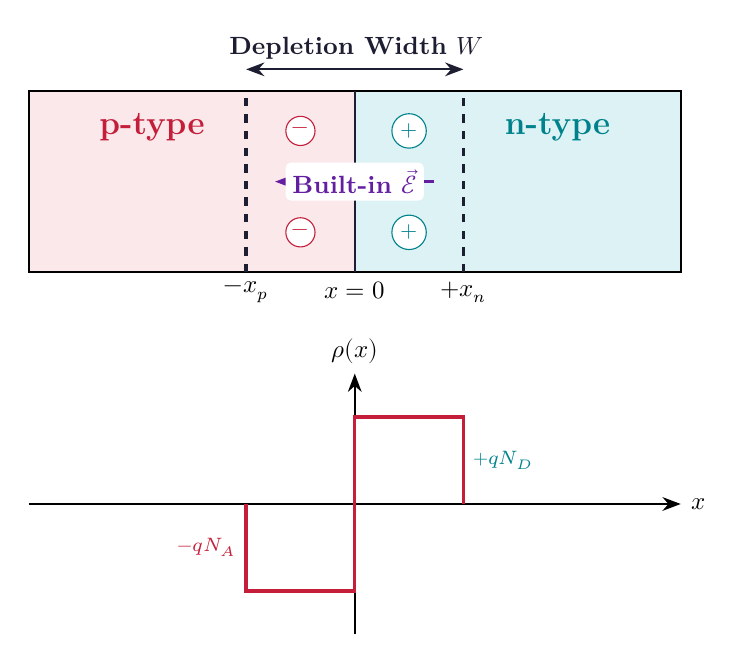
\begin{tikzpicture}[scale=0.92]
  % P and N regions
  \draw[thick, fill=hdrred] (-4.5, 0) rectangle (0, 2.5);
  \draw[thick, fill=hdrteal] (0, 0) rectangle (4.5, 2.5);
  \node[font=\large\bfseries\color{myred}] at (-2.8, 2.0) {p-type};
  \node[font=\large\bfseries\color{myteal}] at (2.8, 2.0) {n-type};

  % Depletion boundaries
  \draw[dashed, very thick, color=mydark] (-1.5, 0) -- (-1.5, 2.5);
  \draw[dashed, very thick, color=mydark] (1.5, 0) -- (1.5, 2.5);
  \draw[thick, color=mydark] (0, 0) -- (0, 2.5);

  % Immobile ions
  \foreach \y in {0.55, 1.95} {
    \node[draw=myred, circle, inner sep=1.5pt, fill=white, font=\footnotesize\bfseries\color{myred}] at (-0.75, \y) {$-$};
    \node[draw=myteal, circle, inner sep=1.5pt, fill=white, font=\footnotesize\bfseries\color{myteal}] at (0.75, \y) {$+$};
  }

  % Electric field vector
  \draw[-Stealth, very thick, color=mypurple] (1.1, 1.25) -- (-1.1, 1.25) node[midway, fill=white, inner sep=2.5pt, rounded corners=2pt, font=\small\bfseries\color{mypurple}] {Built-in $\vec{\mathcal{E}}$};

  % Labels
  \node[below, font=\small] at (-1.5, 0) {$-x_p$};
  \node[below, font=\small] at (0, 0) {$x=0$};
  \node[below, font=\small] at (1.5, 0) {$+x_n$};
  \draw[Stealth-Stealth, thick, color=mydark] (-1.5, 2.8) -- (1.5, 2.8) node[midway, above, font=\small\bfseries] {Depletion Width $W$};

  % Space charge density plot rho(x)
  \begin{scope}[yshift=-3.2cm]
    \draw[-Stealth, thick] (-4.5, 0) -- (4.5, 0) node[right, font=\small] {$x$};
    \draw[-Stealth, thick] (0, -1.8) -- (0, 1.8) node[above, font=\small] {$\rho(x)$};
    \draw[very thick, color=myred] (-1.5, 0) -- (-1.5, -1.2) -- (0, -1.2) -- (0, 1.2) -- (1.5, 1.2) -- (1.5, 0);
    \node[left, font=\scriptsize\bfseries\color{myred}] at (-1.5, -0.6) {$-q N_A$};
    \node[right, font=\scriptsize\bfseries\color{myteal}] at (1.5, 0.6) {$+q N_D$};
  \end{scope}
\end{tikzpicture}
\end{tcolorbox}

\subsection{Derivation of the Built-In Potential (\texorpdfstring{$V_{bi}$}{Vbi})}
Under thermal equilibrium, setting the hole current density to zero:
\begin{align}
  J_p = q p \mu_p \mathcal{E} - q D_p \frac{dp}{dx} &= 0 \\
  \mu_p \mathcal{E} &= D_p \frac{1}{p} \frac{dp}{dx}
\end{align}

Using the Einstein relation $\frac{D_p}{\mu_p} = \frac{kT}{q} = V_T$ and the electrostatic relation $\mathcal{E} = -\frac{dV}{dx}$:
\begin{equation}
  -\frac{dV}{dx} = \frac{k T}{q} \frac{1}{p} \frac{dp}{dx} \implies -dV = \frac{k T}{q} \frac{dp}{p}
\end{equation}

Integrating from the neutral p-region ($x = -x_p$, where $p = p_{p0} \approx N_A$ and $V = 0$) to the neutral n-region ($x = x_n$, where $p = p_{n0} = n_i^2/N_D$ and $V = V_{bi}$):
\begin{equation}
  -\int_0^{V_{bi}} dV = \frac{k T}{q} \int_{p_{p0}}^{p_{n0}} \frac{dp}{p}
\end{equation}
\begin{equation}
  -V_{bi} = \frac{k T}{q} \ln\left(\frac{p_{n0}}{p_{p0}}\right) = -\frac{k T}{q} \ln\left(\frac{p_{p0}}{p_{n0}}\right)
\end{equation}

Substituting $p_{p0} \approx N_A$ and $p_{n0} = \frac{n_i^2}{N_D}$:

\begin{tcolorbox}[formulabox, title={\textbf{Built-In Potential (Contact Potential)}}]
\begin{equation}
  V_{bi} = V_T \ln\left(\frac{N_A N_D}{n_i^2}\right) = \frac{k T}{q} \ln\left(\frac{N_A N_D}{n_i^2}\right)
\end{equation}
At $T = 300\,\text{K}$ ($V_T \approx 25.9\,\text{mV}$), for Silicon with $N_A = 10^{16}\,\text{cm}^{-3}, N_D = 10^{17}\,\text{cm}^{-3}$:
$V_{bi} \approx 0.0259 \ln\left(\frac{10^{33}}{2.25 \times 10^{20}}\right) \approx 0.75\,\text{V}$.
\end{tcolorbox}

\subsection{Depletion Width and Electric Field Analysis}
By integrating Poisson's equation $\frac{d\mathcal{E}}{dx} = \frac{\rho(x)}{\epsilon_s}$ across an abrupt step junction:
\begin{itemize}[leftmargin=*, itemsep=2pt]
  \item For $-x_p \le x \le 0$: $\mathcal{E}(x) = -\frac{q N_A}{\epsilon_s} (x + x_p)$
  \item For $0 \le x \le x_n$: $\mathcal{E}(x) = +\frac{q N_D}{\epsilon_s} (x - x_n)$
\end{itemize}

By overall charge neutrality, the total negative space charge must balance the positive space charge:
\begin{equation}
  q N_A x_p = q N_D x_n \implies \frac{x_n}{x_p} = \frac{N_A}{N_D}
\end{equation}
The depletion region penetrates deeper into the more lightly doped semiconductor side.

\begin{tcolorbox}[formulabox, title={\textbf{Depletion Width and Peak Electric Field under Applied Bias $V_a$}}]
For an applied voltage $V_a$ ($V_a > 0$ for forward bias, $V_a = -V_R$ for reverse bias):
\begin{equation}
  W = x_n + x_p = \sqrt{\frac{2 \epsilon_s}{q} \left(\frac{1}{N_A} + \frac{1}{N_D}\right) (V_{bi} - V_a)}
\end{equation}
Individual depletion layer penetrations:
\begin{equation}
  x_n = W \left(\frac{N_A}{N_A + N_D}\right), \qquad x_p = W \left(\frac{N_D}{N_A + N_D}\right)
\end{equation}
The maximum electric field occurs at the metallurgical junction ($x = 0$):
\begin{equation}
  \mathcal{E}_{\text{max}} = -\frac{2 (V_{bi} - V_a)}{W} = -\frac{q N_D x_n}{\epsilon_s} = -\frac{q N_A x_p}{\epsilon_s}
\end{equation}
\end{tcolorbox}

\subsection{Energy Band Diagrams under Bias}
\begin{itemize}[leftmargin=*, itemsep=3pt]
  \item \textbf{Thermal Equilibrium ($V_a = 0$):} The Fermi level is flat throughout the entire device ($dE_F/dx = 0$). The total band bending is equal to the built-in potential barrier: $q V_{bi}$.
  \item \textbf{Forward Bias ($V_a > 0$):} Positive terminal connected to p-side, negative to n-side. The potential barrier is reduced to $q(V_{bi} - V_a)$. Depletion width narrows, and the Fermi level splits into two separate \textbf{quasi-Fermi levels}: $E_{Fn} - E_{Fp} = q V_a$. Majority carriers readily diffuse across the lowered barrier.
  \item \textbf{Reverse Bias ($V_a = -V_R < 0$):} Positive terminal connected to n-side, negative to p-side. The potential barrier increases to $q(V_{bi} + V_R)$. Depletion width expands, completely blocking majority diffusion. Only thermally generated minority carriers drift across the junction, producing a tiny saturation current $I_0$.
\end{itemize}

% ===============================================================================
\section{P-N Junction Fabrication Technologies}
% ===============================================================================

Modern semiconductor devices are fabricated using planar integrated circuit technologies:

\par\vspace{6pt}\noindent
\begingroup
\setlength{\tabcolsep}{5pt}
\setlength{\extrarowheight}{3pt}
\renewcommand{\arraystretch}{1.35}
\begin{tabularx}{\linewidth}{|B{3.2cm}|Y|Y|}
\hline
\multicolumn{1}{|c|}{\textbf{Method}} & \multicolumn{1}{c|}{\textbf{Process Description}} & \multicolumn{1}{c|}{\textbf{Key Characteristics}} \\
\hline
Grown Junction & Dopant impurities are introduced into the molten melt during crystal pulling (Czochralski process). & Historical method; poor dimensional control; abruptness limited. \\
\hline
Alloyed Junction & A pellet of trivalent impurity (e.g., Indium) is melted onto an n-type substrate and recrystallized. & Forms extremely abrupt junctions; rugged; large junction depth variations. \\
\hline
Thermal Diffusion & Dopant vapor is diffused at elevated temperatures ($900\text{--}1200^\circ\text{C}$) into masked wafer windows. & Planar geometry; excellent reproducibility; lateral diffusion under oxide masks occurs. \\
\hline
Ion Implantation & Dopant ions are ionized, accelerated to high energies ($10\text{--}400\,\text{keV}$), and fired into the wafer. & Precise dosage and depth profile control; low processing temperature; requires thermal annealing to heal crystal damage. \\
\hline
Epitaxial Growth & High-purity single-crystal layer grown on single-crystal substrate using Chemical Vapor Deposition (CVD). & Controlled uniform thickness and doping; used for collector layers and buried layers. \\
\hline
\end{tabularx}
\endgroup

% ===============================================================================
\section{I-V Characteristics and Small Signal Switching Models}
% ===============================================================================

\subsection{The Shockley Diode Equation}
Under the assumption of low-level injection and steady-state conditions, the current flowing through a p-n junction diode is given by the \textbf{Shockley Ideal Diode Equation}:

\begin{tcolorbox}[formulabox, title={\textbf{Shockley Diode Equation and Reverse Saturation Current}}]
\begin{equation}
  I = I_0 \left[ \exp\left(\frac{q V_a}{\eta k T}\right) - 1 \right] = I_0 \left[ \exp\left(\frac{V_a}{\eta V_T}\right) - 1 \right]
\end{equation}
where $\eta$ is the \textbf{ideality factor} ($\eta \approx 1$ for Germanium; $\eta \approx 2$ at low current in Silicon where depletion recombination dominates, and $\eta \approx 1$ at higher forward currents where diffusion dominates).

The \textbf{reverse saturation current} $I_0$ is:
\begin{equation}
  I_0 = q A \left( \frac{D_p p_{n0}}{L_p} + \frac{D_n n_{p0}}{L_n} \right) = q A n_i^2 \left( \frac{D_p}{L_p N_D} + \frac{D_n}{L_n N_A} \right)
\end{equation}
Because $I_0 \propto n_i^2 \propto T^3 \exp(-E_g / kT)$, $I_0$ is extremely temperature-sensitive:
\begin{itemize}[leftmargin=*, itemsep=2pt, topsep=0pt]
  \item $I_0$ approximately \textbf{doubles for every $10^\circ\text{C}$ rise} in temperature for Silicon.
  \item Forward voltage drop decreases by approximately $\mathbf{-2\,\text{mV/}^\circ\text{C}}$ for a constant forward current.
\end{itemize}
\end{tcolorbox}

\subsection{Small-Signal AC Model of P-N Diode}
When a small sinusoidal AC signal ($v_d \ll V_T$) is superimposed on a DC operating point ($V_D, I_D$):

\begin{enumerate}[label=\arabic*., leftmargin=*]
  \item \textbf{Dynamic (AC) Resistance ($r_d$):} The slope of the forward I-V characteristic:
  \begin{equation}
    r_d = \left(\frac{dI}{dV}\right)^{-1} = \frac{\eta V_T}{I_D + I_0} \approx \frac{\eta V_T}{I_D}
  \end{equation}
  At $I_D = 1\,\text{mA}$, for $\eta = 1$: $r_d \approx \frac{25.9\,\text{mV}}{1\,\text{mA}} \approx 26\,\Omega$.

  \item \textbf{Junction (Depletion) Capacitance ($C_j$):} Arises from dipole charge variation ($dQ/dV$) stored in the uncompensated depletion region under reverse bias:
  \begin{equation}
    C_j = \frac{\epsilon_s A}{W} = \frac{C_{j0}}{\left(1 + \displaystyle\frac{V_R}{V_{bi}}\right)^m}
  \end{equation}
  where $m = 1/2$ for an abrupt (step) junction, and $m = 1/3$ for a linearly graded junction. Dominates under \textbf{reverse bias}.

  \item \textbf{Diffusion Capacitance ($C_d$):} Arises from the rearrangement of injected excess minority carrier charge stored in the neutral regions under forward bias:
  \begin{equation}
    C_d = \frac{d Q_{\text{diff}}}{d V_a} = \frac{d (I_D \tau_T)}{d V_a} = \tau_T \frac{d I_D}{d V_a} = \frac{\tau_T I_D}{\eta V_T}
  \end{equation}
  where $\tau_T$ is the minority carrier transit time. $C_d$ is directly proportional to forward current $I_D$ and dominates heavily under \textbf{forward bias}.
\end{enumerate}

\subsection{Diode Switching Characteristics and Reverse Recovery Time}
When a diode is switched rapidly from forward conduction ($I_F$) to reverse bias ($-V_R$):

\begin{itemize}[leftmargin=*, itemsep=3pt]
  \item The diode cannot turn off instantaneously because a substantial amount of excess minority carrier charge $Q_s = I_F \tau_T$ is stored in the neutral base.
  \item \textbf{Storage Time ($t_s$):} The time required to extract the stored excess charge near the junction until the carrier density drops to equilibrium. Current remains high and negative ($I_R \approx -V_R / R_L$).
  \item \textbf{Transition Time ($t_t$):} The time required for the junction depletion layer capacitance to charge up to the reverse bias voltage $-V_R$. Current decays asymptotically to $-I_0$.
  \item \textbf{Reverse Recovery Time ($t_{rr}$):} Total turn-off time:
  \begin{equation}
    t_{rr} = t_s + t_t
  \end{equation}
\end{itemize}

% ===============================================================================
\section{Junction Breakdown Mechanisms and Diodes}
% ===============================================================================

When a sufficiently large reverse bias voltage ($V_R = V_{BR}$) is applied across a p-n junction, the reverse current increases drastically with negligible increase in voltage.

\subsection{Zener Breakdown vs. Avalanche Breakdown}
\par\vspace{6pt}\noindent
\begingroup
\setlength{\tabcolsep}{5pt}
\setlength{\extrarowheight}{3pt}
\renewcommand{\arraystretch}{1.35}
\begin{tabularx}{\linewidth}{|B{3.2cm}|Y|Y|}
\hline
\multicolumn{1}{|c|}{\textbf{Parameter}} & \multicolumn{1}{c|}{\textbf{Zener Breakdown}} & \multicolumn{1}{c|}{\textbf{Avalanche Breakdown}} \\
\hline
Doping Concentration & Heavily doped on both p and n sides ($N_A, N_D > 10^{18}\,\text{cm}^{-3}$) & Lightly to moderately doped ($N_A, N_D < 10^{16}\,\text{cm}^{-3}$) \\
\hline
Depletion Width ($W$) & Extremely thin ($W < 10\,\text{nm} = 100\,\text{\AA}$) & Relatively wide ($W > 1\,\mu\text{m}$) \\
\hline
Breakdown Voltage ($V_{BR}$) & Occurs at low reverse voltages ($V_{BR} < 4\text{--}6\,\text{V}$) & Occurs at higher reverse voltages ($V_{BR} > 6\,\text{V}$) \\
\hline
Physical Mechanism & Direct quantum mechanical tunneling of valence electrons from p-side VB to n-side CB across thin barrier & Impact ionization: high kinetic energy carriers collide with lattice atoms, generating secondary EHPs (avalanche multiplication) \\
\hline
Electric Field & High electric field ($\mathcal{E} \ge 10^6\,\text{V/cm}$) & Moderate to high field ($\mathcal{E} \sim 2\text{--}4 \times 10^5\,\text{V/cm}$) \\
\hline
Temperature Coefficient & \textbf{Negative:} As $T$ rises, bandgap $E_g$ narrows, making tunneling easier $\implies V_Z$ decreases & \textbf{Positive:} As $T$ rises, lattice vibrations increase, shortening mean free path, requiring higher voltage for collision ionization $\implies V_A$ increases \\
\hline
\end{tabularx}
\endgroup

\subsection{Schottky Diode (Metal-Semiconductor Junction)}
A \textbf{Schottky barrier diode} is formed by depositing a metal (e.g., Gold, Platinum, Tungsten, Aluminum) directly onto an n-type semiconductor.

\begin{itemize}[leftmargin=*, itemsep=3pt]
  \item \textbf{Schottky Barrier Height ($\Phi_B$):}
  \begin{equation}
    \Phi_B = \Phi_m - \chi_s
  \end{equation}
  where $\Phi_m$ is the metal work function, and $\chi_s$ is the semiconductor electron affinity.
  \item \textbf{Built-in Potential ($V_{bi}$):}
  \begin{equation}
    V_{bi} = \Phi_B - (E_c - E_F) / q
  \end{equation}
  \item \textbf{Majority Carrier Conduction:} Current conduction occurs entirely via majority electron \textbf{thermionic emission} over the barrier into the metal.
  \item \textbf{Zero Minority Storage Time:} Because there is virtually no minority carrier injection into the semiconductor, there is zero stored charge ($Q_s \approx 0$). The reverse recovery time $t_{rr}$ is virtually zero ($\sim 10\text{--}100\,\text{ps}$), making Schottky diodes ideal for high-speed switching and ultra-high frequency (RF/microwave) clamping circuits.
  \item \textbf{Low Cut-In Voltage:} The forward knee voltage is only $0.2\text{--}0.3\,\text{V}$ (compared to $0.7\,\text{V}$ for Silicon p-n diodes).
\end{itemize}

% ===============================================================================
\section{Bipolar Junction Transistor (BJT)}
% ===============================================================================

The Bipolar Junction Transistor is a three-terminal, two-junction semiconductor device whose operation depends on both majority and minority carrier transport (hence \textbf{bipolar}).

\subsection{Basic Construction and Doping Asymmetry}
A BJT consists of three alternating regions: Emitter ($E$), Base ($B$), and Collector ($C$), forming an n-p-n or p-n-p sandwich:

\par\vspace{6pt}\noindent
\begingroup
\setlength{\tabcolsep}{3.5pt}
\setlength{\extrarowheight}{3pt}
\renewcommand{\arraystretch}{1.35}
\begin{tabularx}{\linewidth}{|B{2.2cm}|Y|Y|Y|}
\hline
\textbf{Region} & \textbf{Doping Concentration} & \textbf{Physical Width} & \textbf{Primary Functional Role} \\
\hline
Emitter ($E$) & Heavily doped ($N_E \approx 10^{19}\,\text{cm}^{-3}$) & Moderate & Injects majority carriers into the base with maximum injection efficiency. \\
\hline
Base ($B$) & Very lightly doped ($N_B \approx 10^{16}\,\text{cm}^{-3}$) & Extremely narrow ($W_b \ll L_{\text{minority}}$) & Transports injected minority carriers to the collector with minimum recombination. \\
\hline
Collector ($C$) & Moderately / Lightly doped ($N_C \approx 10^{15}\,\text{cm}^{-3}$) & Largest physical dimensions & Collects carriers sweeping across reverse-biased CB junction; dissipates heat. \\
\hline
\end{tabularx}
\endgroup

\subsection{BJT Operating Modes}
\par\vspace{6pt}\noindent
\begingroup
\setlength{\tabcolsep}{3.5pt}
\setlength{\extrarowheight}{3pt}
\renewcommand{\arraystretch}{1.35}
\begin{tabularx}{\linewidth}{|B{2.3cm}|Y|Y|Y|}
\hline
\textbf{Operating Mode} & \textbf{Emitter-Base Junction (EBJ)} & \textbf{Collector-Base Junction (CBJ)} & \textbf{Primary Application} \\
\hline
Forward Active & Forward Biased & Reverse Biased & Linear analog amplification \\
\hline
Cut-off & Reverse Biased & Reverse Biased & Digital logic ``OFF'' switch ($I_C \approx 0$) \\
\hline
Saturation & Forward Biased & Forward Biased & Digital logic ``ON'' switch ($V_{CE,\text{sat}} \approx 0.2\,\text{V}$) \\
\hline
Inverse / Inverted & Reverse Biased & Forward Biased & Specialized bidirectional switching \\
\hline
\end{tabularx}
\endgroup

\subsection{Current Relationships in Forward Active Mode}
For an n-p-n transistor in forward active mode:
\begin{enumerate}[label=\arabic*., leftmargin=*]
  \item Electrons injected from Emitter into Base form emitter current $I_E$.
  \item A tiny fraction ($< 1\%$) recombines with holes in the thin base, forming base current $I_B$.
  \item The remaining vast majority ($> 99\%$) diffuses across the neutral base, reaches the CB depletion edge, and is swept into the collector by the strong reverse electric field, forming collector current $I_C$:
\end{enumerate}

\begin{tcolorbox}[formulabox, title={\textbf{BJT Current Relationships}}]
\begin{equation}
  I_E = I_B + I_C
\end{equation}
Common-Base Current Gain ($\alpha$):
\begin{equation}
  \alpha = \frac{I_C}{I_E} \approx 0.95 \text{ to } 0.998
\end{equation}
Common-Emitter Current Gain ($\beta$ or $h_{FE}$):
\begin{equation}
  \beta = \frac{I_C}{I_B} = \frac{\alpha}{1 - \alpha} \approx 50 \text{ to } 500
\end{equation}
In terms of reverse collector saturation current ($I_{CBO}$):
\begin{equation}
  I_C = \alpha I_E + I_{CBO} = \beta I_B + (\beta + 1) I_{CBO} = \beta I_B + I_{CEO}
\end{equation}
\end{tcolorbox}

\subsection{Base Width Modulation (The Early Effect)}
In forward active mode, as the reverse bias voltage across the collector-base junction ($V_{CB}$ or $V_{CE}$) increases:
\begin{itemize}[leftmargin=*, itemsep=3pt]
  \item The collector-base space charge region expands into the lightly doped base.
  \item The \textbf{effective neutral base width} ($W_{\text{eff}} = W_{\text{base}} - x_{p,\text{dep}}$) decreases.
  \item \textbf{Consequences}:
    \begin{enumerate}
      \item Less recombination in the base $\implies$ Base transport factor increases $\implies \alpha$ and $\beta$ increase.
      \item The concentration gradient of minority electrons in the base ($dn/dx \approx n(0)/W_{\text{eff}}$) steepens $\implies I_C$ increases with increasing $V_{CE}$.
    \end{enumerate}
  \item When extrapolated backward, the linear output characteristics in the active region intersect the negative voltage axis at a common voltage called the \textbf{Early Voltage} ($V_A \approx 50\text{--}100\,\text{V}$).
  \item The collector current incorporating the Early effect is modeled as:
  \begin{equation}
    I_C = I_S \exp\left(\frac{V_{BE}}{V_T}\right) \left( 1 + \frac{V_{CE}}{V_A} \right)
  \end{equation}
  yielding a finite small-signal output resistance: $r_o = \frac{V_A + V_{CE}}{I_C} \approx \frac{V_A}{I_C}$.
\end{itemize}

\subsection{BJT I-V Characteristics (Common-Emitter Input and Output)}
The static electrical behavior of a BJT in the Common-Emitter (CE) configuration is described by two sets of characteristic curves:

\begin{enumerate}[label=\arabic*., leftmargin=*]
  \item \textbf{Input Characteristics ($I_B$ vs. $V_{BE}$ for constant $V_{CE}$):}
  \begin{itemize}
    \item Resembles the exponential forward $I\text{-}V$ curve of a p-n junction diode with knee / cut-in voltage $V_\gamma \approx 0.6\text{--}0.7\,\text{V}$ for Silicon.
    \item As $V_{CE}$ increases, base width modulation (Early effect) narrows the effective base width $W_{\text{eff}}$, reducing base recombination. Consequently, a higher $V_{BE}$ is required to sustain the same base current $I_B$, shifting the curve slightly to the right.
    \item \textbf{Dynamic Input Resistance:} $h_{ie} = r_\pi = \left.\frac{\partial V_{BE}}{\partial I_B}\right|_{V_{CE} = \text{const}} \approx 1\text{ to } 5\,\text{k}\Omega$.
  \end{itemize}
  \item \textbf{Output Characteristics ($I_C$ vs. $V_{CE}$ for constant $I_B$):}
  Displays four distinct regions of transistor operation:
  \begin{itemize}
    \item \textbf{Cut-off Region ($I_B \le 0$):} Both EBJ and CBJ are reverse-biased. The transistor is turned OFF, with only a negligible leakage current flowing: $I_C = I_{CEO} = (\beta + 1)I_{CBO} \approx 0$.
    \item \textbf{Saturation Region ($0 \le V_{CE} \le V_{CE,\text{sat}} \approx 0.2\,\text{V}$):} Both EBJ and CBJ are forward-biased. $I_C$ increases rapidly and linearly with $V_{CE}$, limited only by external circuit load ($I_{C,\text{sat}} \approx V_{CC}/R_C$), independent of $I_B$ ($I_C < \beta I_B$).
    \item \textbf{Active Region ($V_{CE} > 0.2\,\text{V}$, $I_B > 0$):} EBJ is forward-biased and CBJ is reverse-biased. The collector current is controlled primarily by the base current ($I_C \approx \beta I_B$). Curves exhibit a slight positive slope due to Early effect, with an output resistance $r_o = \left.\frac{\partial V_{CE}}{\partial I_C}\right|_{I_B} \approx \frac{V_A}{I_C} \approx 40\text{--}100\,\text{k}\Omega$.
    \item \textbf{Avalanche Breakdown Region ($V_{CE} > BV_{CEO}$):} The reverse-biased CB junction enters avalanche multiplication, causing $I_C$ to rise steeply and destructively.
  \end{itemize}
\end{enumerate}

\begin{tcolorbox}[tikzbox, title={Common-Emitter (CE) Output Characteristics ($I_C$ vs. $V_{CE}$)}]
\centering
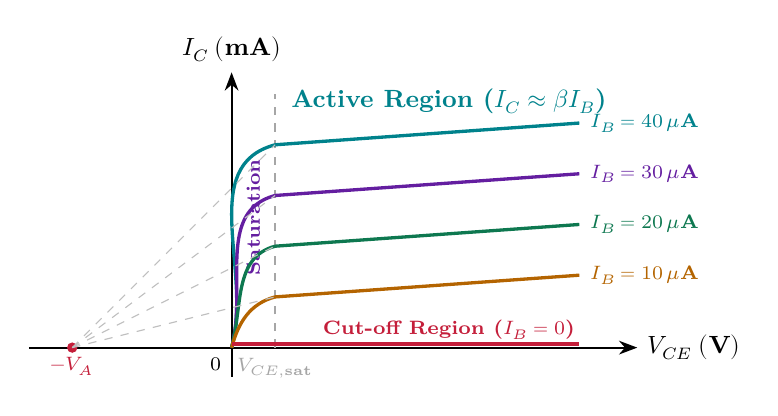
\begin{tikzpicture}[scale=0.92]
  % Axes
  \draw[-Stealth, thick] (-2.8, 0) -- (5.6, 0) node[right, font=\small\bfseries] {$V_{CE}\;(\text{V})$};
  \draw[-Stealth, thick] (0, -0.4) -- (0, 3.8) node[above, font=\small\bfseries] {$I_C\;(\text{mA})$};
  \node[below left, font=\scriptsize] at (0,0) {$0$};

  % Saturation boundary line
  \draw[dashed, thick, color=gray!70] (0.6, 0) node[below, font=\scriptsize\bfseries\color{mydark}] {$V_{CE,\text{sat}}$} -- (0.6, 3.5);

  % Region labels
  \node[font=\scriptsize\bfseries\color{mypurple}, rotate=90] at (0.3, 1.8) {Saturation};
  \node[font=\small\bfseries\color{myteal}] at (3.0, 3.4) {Active Region ($I_C \approx \beta I_B$)};
  \node[font=\scriptsize\bfseries\color{myred}] at (3.0, 0.25) {Cut-off Region ($I_B = 0$)};

  % Early voltage extrapolation point
  \filldraw[color=myred] (-2.2, 0) circle (1.8pt) node[below, font=\scriptsize\bfseries\color{myred}] {$-V_A$};

  % I_B curves
  \foreach \ib/\yc/\col in {40/2.8/myteal, 30/2.1/mypurple, 20/1.4/mygreen, 10/0.7/myamber} {
    \draw[very thick, color=\col] (0,0) to[out=75, in=195] (0.6, \yc);
    \draw[very thick, color=\col] (0.6, \yc) -- (4.8, \yc + 0.3) node[right, font=\scriptsize\bfseries] {$I_B = \ib\,\mu\text{A}$};
    \draw[dashed, thin, color=gray!50] (-2.2, 0) -- (0.6, \yc);
  }

  % Cut-off curve
  \draw[very thick, color=myred] (0, 0.05) -- (4.8, 0.05);
\end{tikzpicture}
\end{tcolorbox}

% ===============================================================================
\section{The Ebers-Moll Model}
% ===============================================================================

The \textbf{Ebers-Moll model} is a generalized, physics-based, large-signal non-linear equivalent circuit model for the BJT valid across \textbf{all four operating modes} (Active, Cut-off, Saturation, and Inverted).

\subsection{Model Formulation and Equivalent Circuit}
The BJT is modeled as two coupled p-n junction diodes connected back-to-back with two current-controlled current sources representing the transistor action:

\begin{itemize}[leftmargin=*, itemsep=3pt]
  \item An Emitter diode carrying current $I_F$ with a dependent collector current source $\alpha_F I_F$.
  \item A Collector diode carrying current $I_R$ with a dependent emitter current source $\alpha_R I_R$.
\end{itemize}

where:
\begin{align}
  I_F &= I_{ES} \left[ \exp\left(\frac{q V_{BE}}{k T}\right) - 1 \right] \\
  I_R &= I_{CS} \left[ \exp\left(\frac{q V_{BC}}{k T}\right) - 1 \right]
\end{align}
$I_{ES}$ and $I_{CS}$ are the saturation currents of the Emitter-Base and Collector-Base junctions, respectively, and $\alpha_F$ ($\alpha_{\text{forward}}$) and $\alpha_R$ ($\alpha_{\text{reverse}}$) are the forward and reverse common-base current gains.

\begin{tcolorbox}[formulabox, title={\textbf{Ebers-Moll Equations}}]
The terminal currents for an n-p-n transistor are:
\begin{align}
  I_E &= I_F - \alpha_R I_R = I_{ES} \left( e^{V_{BE}/V_T} - 1 \right) - \alpha_R I_{CS} \left( e^{V_{BC}/V_T} - 1 \right) \\
  I_C &= \alpha_F I_F - I_R = \alpha_F I_{ES} \left( e^{V_{BE}/V_T} - 1 \right) - I_{CS} \left( e^{V_{BC}/V_T} - 1 \right) \\
  I_B &= I_E - I_C = (1 - \alpha_F) I_F + (1 - \alpha_R) I_R
\end{align}
\textbf{The Reciprocity Condition:} By thermodynamic reciprocity of linear carrier diffusion across the base:
\begin{equation}
  \alpha_F I_{ES} = \alpha_R I_{CS} = I_S
\end{equation}
where $I_S$ is the fundamental BJT saturation transfer current.
\end{tcolorbox}

\begin{tcolorbox}[tikzbox, title={Ebers-Moll Large-Signal Equivalent Circuit (N-P-N Transistor)}]
\centering
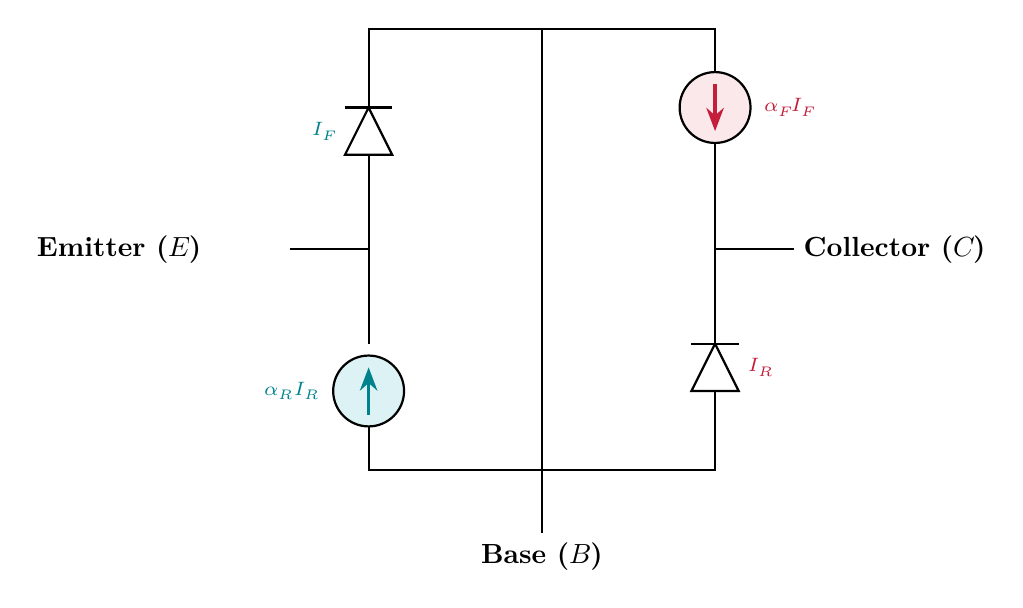
\begin{tikzpicture}[scale=1.0]
  % Emitter Terminal
  \node[left, font=\normalsize\bfseries] at (-4.2, 0) {Emitter ($E$)};
  \draw[thick] (-3.2, 0) -- (-2.2, 0);

  % Forward Diode
  \draw[thick] (-2.2, 0) -- (-2.2, 1.2);
  \draw[thick] (-2.5, 1.2) -- (-1.9, 1.2) -- (-2.2, 1.8) -- cycle;
  \draw[thick] (-2.5, 1.8) -- (-1.9, 1.8);
  \draw[thick] (-2.2, 1.8) -- (-2.2, 2.8) -- (0, 2.8);
  \node[left, font=\scriptsize\bfseries\color{myteal}] at (-2.5, 1.5) {$I_F$};

  % Reverse Current Source alpha_R * I_R
  \draw[thick] (-2.2, 0) -- (-2.2, -1.2);
  \draw[thick, fill=hdrteal] (-2.2, -1.8) circle (0.45);
  \draw[-Stealth, very thick, color=myteal] (-2.2, -2.1) -- (-2.2, -1.5);
  \node[left, font=\scriptsize\bfseries\color{myteal}] at (-2.7, -1.8) {$\alpha_R I_R$};
  \draw[thick] (-2.2, -2.25) -- (-2.2, -2.8) -- (0, -2.8);

  % Base Terminal
  \draw[thick] (0, 2.8) -- (0, -2.8);
  \draw[thick] (0, 0) -- (0, -3.6) node[below, font=\normalsize\bfseries] {Base ($B$)};

  % Forward Current Source alpha_F * I_F
  \draw[thick] (0, 2.8) -- (2.2, 2.8) -- (2.2, 2.25);
  \draw[thick, fill=hdrred] (2.2, 1.8) circle (0.45);
  \draw[-Stealth, very thick, color=myred] (2.2, 2.1) -- (2.2, 1.5);
  \node[right, font=\scriptsize\bfseries\color{myred}] at (2.7, 1.8) {$\alpha_F I_F$};
  \draw[thick] (2.2, 1.35) -- (2.2, 0);

  % Reverse Diode
  \draw[thick] (0, -2.8) -- (2.2, -2.8) -- (2.2, -1.8);
  \draw[thick] (1.9, -1.8) -- (2.5, -1.8) -- (2.2, -1.2) -- cycle;
  \draw[thick] (1.9, -1.2) -- (2.5, -1.2);
  \draw[thick] (2.2, -1.2) -- (2.2, 0);
  \node[right, font=\scriptsize\bfseries\color{myred}] at (2.5, -1.5) {$I_R$};

  % Collector Terminal
  \draw[thick] (2.2, 0) -- (3.2, 0);
  \node[right, font=\normalsize\bfseries] at (3.2, 0) {Collector ($C$)};
\end{tikzpicture}
\end{tcolorbox}

\newpage
% ===============================================================================
% MANDATORY QUICK REVISION PAGE
% ===============================================================================
\begin{center}
  {\large\bfseries\color{myred} Quick Revision --- Module 2}\\[3pt]
  {\small\color{mydark} P-N Junction \& Bipolar Junction Transistor $|$ EC301}
\end{center}
\noindent{\color{myred}\rule{\linewidth}{1.2pt}}
\vspace{4pt}

\begin{tcolorbox}[formulabox, title={\textbf{Key Formulas and Metrics at a Glance}}]
\renewcommand{\arraystretch}{1.35}
\begin{tabularx}{\linewidth}{B{5.0cm} X}
Built-in Potential ($V_{bi}$) & $V_{bi} = V_T \ln\left(\frac{N_A N_D}{n_i^2}\right)$ \\[4pt]
Depletion Width ($W$) & $W = \sqrt{\frac{2\epsilon_s}{q}\left(\frac{1}{N_A} + \frac{1}{N_D}\right)(V_{bi} - V_a)}$ \\[4pt]
Maximum Electric Field & $\mathcal{E}_{\text{max}} = -\frac{2(V_{bi} - V_a)}{W} = -\frac{q N_D x_n}{\epsilon_s}$ \\[4pt]
Shockley Diode Equation & $I = I_0 \left[ \exp\left(\frac{V_a}{\eta V_T}\right) - 1 \right]$ \\[4pt]
Dynamic AC Resistance ($r_d$) & $r_d = \frac{\eta V_T}{I_D} \approx \frac{26\,\text{mV}}{I_D}$ \\[4pt]
Junction Capacitance ($C_j$) & $C_j = \frac{\epsilon_s A}{W} \propto (V_{bi} + V_R)^{-1/2}$ \\[4pt]
Diffusion Capacitance ($C_d$) & $C_d = \frac{\tau_T I_D}{\eta V_T}$ \\[4pt]
Common-Base Gain ($\alpha$) & $\alpha = \frac{I_C}{I_E} = \frac{\beta}{\beta + 1}$ \\[4pt]
Common-Emitter Gain ($\beta$) & $\beta = \frac{I_C}{I_B} = \frac{\alpha}{1 - \alpha}$ \\[4pt]
Early Effect Output Resistance & $r_o \approx \frac{V_A}{I_C}$ \\[4pt]
Ebers-Moll Reciprocity & $\alpha_F I_{ES} = \alpha_R I_{CS} = I_S$ \\[4pt]
\end{tabularx}
\end{tcolorbox}

\begin{tcolorbox}[defbox, title={\textbf{One-Line Definitions}}]
\begin{itemize}[leftmargin=*, itemsep=2pt, topsep=0pt]
  \item \textbf{Depletion Region:} A localized space charge region at the p-n metallurgical interface depleted of mobile carriers.
  \item \textbf{Built-in Potential ($V_{bi}$):} The equilibrium potential difference across the junction maintaining balance between drift and diffusion.
  \item \textbf{Zener Breakdown:} Field-induced quantum tunneling of valence electrons across a very thin depletion barrier under reverse bias.
  \item \textbf{Avalanche Breakdown:} Voltage breakdown caused by cumulative impact ionization multiplying carriers in a wider depletion region.
  \item \textbf{Schottky Diode:} A metal-semiconductor rectifying diode with majority carrier transport and zero reverse recovery storage time.
  \item \textbf{Reverse Recovery Time ($t_{rr}$):} Total time ($t_s + t_t$) required to switch a diode from forward conduction to reverse blocking.
  \item \textbf{Early Effect:} Base-width narrowing under increasing reverse collector-base bias, raising $\beta$ and output conductance.
  \item \textbf{Ebers-Moll Model:} Large-signal equivalent model coupling forward and reverse diodes to model BJT operation in all four modes.
\end{itemize}
\end{tcolorbox}

\begin{tcolorbox}[exambox, title={\textbf{Frequently Asked / Viva Questions}}]
\begin{enumerate}[topsep=0pt, label=\textbf{Q\arabic*.}, itemsep=5pt]
  \item \Q{Why does the depletion region penetrate deeper into the lightly doped side of an asymmetric p-n junction?}
    By the law of space charge neutrality ($q N_A x_p = q N_D x_n$), the total uncovered charge per unit area on both sides must be equal. Hence, the depletion width ratio is inversely proportional to doping: $x_n / x_p = N_A / N_D$.
  \item \Q{Why is diffusion capacitance $C_d$ negligible under reverse bias while junction capacitance $C_j$ is negligible under forward bias?}
    Under reverse bias, forward current is zero, so no minority carriers are injected into the neutral regions ($C_d \propto I_D \approx 0$). Under forward bias, the massive exponential increase in injected minority carriers makes $C_d$ orders of magnitude larger than $C_j$.
  \item \Q{Compare Zener and Avalanche breakdown on the basis of temperature coefficient.}
    Zener breakdown has a \textbf{negative temperature coefficient} because rising temperature narrows $E_g$, enhancing tunneling. Avalanche breakdown has a \textbf{positive temperature coefficient} because rising temperature increases lattice vibrations, reducing carrier mean free path and requiring higher voltage for collision ionization.
  \item \Q{What are the major advantages of a Schottky diode over a standard p-n junction diode?}
    \begin{itemize}[leftmargin=*, itemsep=1pt, topsep=2pt]
      \item Virtually zero minority carrier storage time ($t_{rr} \approx 0$), enabling ultra-high speed switching (GHz range).
      \item Lower forward cut-in voltage ($0.2\text{--}0.3\,\text{V}$ vs $0.7\,\text{V}$), resulting in lower conduction power loss.
    \end{itemize}
  \item \Q{Why must the base of a BJT be made extremely thin and lightly doped?}
    It must be extremely thin ($W_b \ll L_n$) to minimize electron-hole recombination so that almost all injected carriers reach the collector ($I_C \approx I_E$). It must be lightly doped to ensure high emitter injection efficiency ($\gamma \to 1$).
  \item \Q{Explain the physical phenomenon of Early Effect in a BJT.}
    Increasing $V_{CB}$ widens the collector-base depletion layer, which shrinks the effective neutral base width $W_{\text{eff}}$. This increases the base minority concentration gradient, reduces base recombination, and causes collector current $I_C$ to rise with $V_{CE}$.
  \item \Q{What is the reciprocity relation in the Ebers-Moll model?}
    $\alpha_F I_{ES} = \alpha_R I_{CS} = I_S$. It states that the forward and reverse transfer saturation currents across the base are identical, stemming from the reciprocity of minority carrier diffusion across the base.
  \item \Q{What are the conditions on junction biases for a BJT to operate as a closed digital switch (saturation)?}
    Both the Emitter-Base Junction (EBJ) and the Collector-Base Junction (CBJ) must be forward biased ($V_{BE} \approx 0.7\text{--}0.8\,\text{V}, V_{BC} \approx 0.5\text{--}0.6\,\text{V}$), yielding $V_{CE,\text{sat}} \approx 0.2\,\text{V}$.
  \item \Q{How does the reverse saturation current $I_0$ of a Silicon diode vary with temperature?}
    $I_0$ approximately doubles for every $10^\circ\text{C}$ rise in temperature, governed by the exponential temperature dependence of $n_i^2 \propto T^3 \exp(-E_g / kT)$.
  \item \Q{What is the ideality factor $\eta$ in the diode equation?}
    $\eta$ accounts for the dominant recombination/generation mechanism. $\eta \approx 1$ when diffusion current dominates (high forward bias or Germanium), and $\eta \approx 2$ when carrier recombination in the depletion region dominates (low forward bias in Silicon).
\end{enumerate}
\end{tcolorbox}

\begin{tcolorbox}[tikzbox, title={Comparison of BJT Configurations (CB, CE, CC)}]
\centering
\begingroup
\footnotesize
\setlength{\tabcolsep}{3.5pt}
\setlength{\extrarowheight}{2.5pt}
\renewcommand{\arraystretch}{1.35}
\begin{tabularx}{\linewidth}{|>{\raggedright\arraybackslash\bfseries}m{2.3cm}|Y|Y|Y|}
\hline
\textbf{Parameter} & \textbf{Common Base (CB)} & \textbf{Common Emitter (CE)} & \textbf{Common Collector (CC)} \\
\hline
Input / Output Terminals & In: Emitter, Out: Collector & In: Base, Out: Collector & In: Base, Out: Emitter \\
\hline
Current Gain & $\alpha < 1$ ($\approx 0.98$) & $\beta = \alpha/(1-\alpha)$ ($50\text{--}300$) & $\gamma = \beta + 1$ (High) \\
\hline
Voltage Gain & High ($A_v \gg 1$) & High ($A_v \gg 1$) & Unity ($A_v \approx 1$, buffer) \\
\hline
Input Impedance ($Z_{in}$) & Very low ($10\text{--}50\,\Omega$) & Moderate ($1\text{--}5\,\text{k}\Omega$) & Very high ($100\text{--}500\,\text{k}\Omega$) \\
\hline
Output Impedance ($Z_{out}$) & Very high ($1\text{--}2\,\text{M}\Omega$) & Moderate ($40\text{--}100\,\text{k}\Omega$) & Very low ($20\text{--}100\,\Omega$) \\
\hline
Phase Shift (In to Out) & $0^\circ$ (In-phase) & $180^\circ$ (Inverted) & $0^\circ$ (In-phase) \\
\hline
Primary Applications & High-frequency RF, current buffer & General voltage \& current amplification & Impedance matching, emitter follower \\
\hline
\end{tabularx}
\endgroup
\end{tcolorbox}

\end{document}
